\documentclass{article}
\usepackage{indentfirst}
\usepackage{ctex}
\usepackage{geometry}
\usepackage{enumerate}
\usepackage{graphicx, subfigure}
\geometry{left=3.17cm,right=3.17cm,top=2.54cm,bottom=2.54cm} % 页边距

\begin{document}

\title{LDA Meets Word2Vec: A Novel Model for Academic Abstract Clustering}
\date{}
\maketitle

\section{INTRODUCTION}
针对学术论文的文本聚类:
\begin{itemize}
	\item 现状:传统的聚类算法在多领域文档集上的应用较为广泛,但是针对窄领域(narrow-domain)文档集(比如全是computer science)的聚类研究比较少。近年来,研究者把更多的注意力放到了它的身上[3,4,5].
	\item 已有的方法:
	\begin{itemize}
		\item 针对部分学术论文无法取得其全文的问题,基于关键词的方法不可行,因为对于窄领域文档集,由于其中大量文档来自相同领域,所以关键词的重叠非常严重,很难通过关键词进行准确区分。
		\item {[5,6]建议使用摘要进行聚类。摘要作为短文本,聚类时面临稀疏性问题。为了解决这一问题,[8,9,10,11]提出了不同的方法,其中最受关注的是LDA模型。[12,13,14,15]都是对LDA的各种应用、扩展。LDA的局限:虽然善于从文本内部抽取出横向主题信息,但是其低维特征削弱了区分文本的能力。}
		\item 窄领域文档集的摘要大量重叠,但摘要一般都包含3个关键信息:研究意图、新方法和结论。基于此,我们提出了Partition Word2Vec-LDA(PW-LDA)模型,用于对摘要进行准确聚类。
	\end{itemize}
	\item 本文的方法:
	\begin{itemize}
		\item 问题:文档所属的领域单一、摘要短小,所以文本信息严重重叠。解决方法:摘要一般都包含3个关键信息:研究意图、新方法和结论,将其抽取出来即可。于是我们提出了Partition Word2Vec-LDA(PW-LDA)模型,用于对摘要进行准确聚类。
		\item 我们没有使用整个摘要,而是从中抽取出3个关键信息对应的句子,然后对其应用LDA和Word2Vec。
		\item {[18]将Word2Vec和LDA结合,通过语义空间中的bag-of-distances从文档中提取特征。该方法结合了文档和主题之间的关系,以及单词之间的语境关系,能取得良好的分类效果。我们受其启发,提出了主题嵌入和句子嵌入,用于度量主题和文档之间的相似度。}
	\end{itemize}
\end{itemize}

\section{METHODOLOGY}
\subsection{Preliminaries}
\subsubsection{LDA}
LDA是一种生成概率主题模型,它将每篇文档表示为潜在主题的随机混合,每个主题表示为固定词集的分布[12]。在LDA中,每篇文档能够以不同的程度显示出多个主题。每篇文档中的单词都是观测数据,根据这一点,LDA的主要目标是推断出潜在的主题结构。对于语料库中的每篇文档,单词的生成需要两个阶段。首先,随机选择一个主题分布。然后,对于文档中的每个单词,从主题分布中随机选择一个主题,再从特定分布中随机选择一个单词。LDA被建模为三层贝叶斯模型,如图\ref{fig:lda_model}。在图\ref{fig:lda_model}中,节点表示随机变量,边表示随机变量之间可能的依赖关系。$\alpha$和$\beta$表示Dirichlet参数,$\theta$表示文档级别的主题变量,$z$表示每个单词的主题分配,$w$表示观测到的单词。$\alpha$和$\beta$取决于主题个数和词汇表大小[12],为每篇文档对文档级别的主题变量进行采样,为文档中的每个单词对单词级别的主题变量进行采样。在LDA中,单词作为词汇表中的离散数据,被标号为$1,\dots,V$. 一篇文档被表示为$N$个单词序列$\textbf{w}=(w_1,w_2,\dots,w_N)$. 一个语料库由$M$篇文档组成,被表示为$D=(\textbf{w}_1,\textbf{w}_2,\dots,\textbf{w}_M)$.\par
在参数求解过程中,$w$表示观测变量,$\theta$和$z$表示隐藏变量。通过应用EM算法,就能学习到$\alpha$和$\beta$.

\begin{figure}[htbp]
	\centering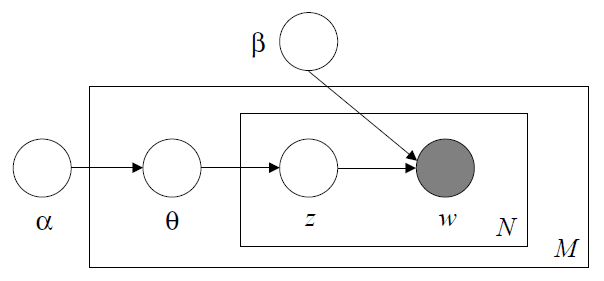
\includegraphics[height=5cm]{lda_model.png}
	\caption{The graphical model of LDA}
	\label{fig:lda_model}
\end{figure}

\end{document}
 